\section{Experiment 1}

write a description of the experiment

write a prediction about the outcomes based off theory

\begin{figure}[H]
        \centering
        \begin{subfigure}[b]{0.475\textwidth}
            \centering
            \includegraphics[width=\textwidth]{./code/Exp1-results/10iters/Train10.png}
            \caption[]%
            {{\small 10 sample training set}}    
            \label{fig:train10}
        \end{subfigure}
        \hfill
        \begin{subfigure}[b]{0.475\textwidth}  
            \centering 
            \includegraphics[width=\textwidth]{./code/Exp1-results/10iters/Train50.png}
            \caption[]%
            {{\small 50 sample training set}}    
            \label{fig:train50}
        \end{subfigure}
        \vskip\baselineskip
        \begin{subfigure}[b]{0.475\textwidth}   
            \centering 
            \includegraphics[width=\textwidth]{./code/Exp1-results/10iters/Train100.png}
            \caption[]%
            {{\small 100 sample training set}}    
            \label{fig:train100}
        \end{subfigure}
        \quad
        \begin{subfigure}[b]{0.475\textwidth}   
            \centering 
            \includegraphics[width=\textwidth]{./code/Exp1-results/10iters/Test100.png}
            \caption[]%
            {{\small 100 sample test set}}    
            \label{fig:test100}
        \end{subfigure}
        \caption[ ]
        {\small Visualisation of examples of test and training data generated for Experiment 1.} 
        \label{fig:SampleDatasets}
    \end{figure}





\subsection{Results}

\begin{figure}[H]
	\centering
	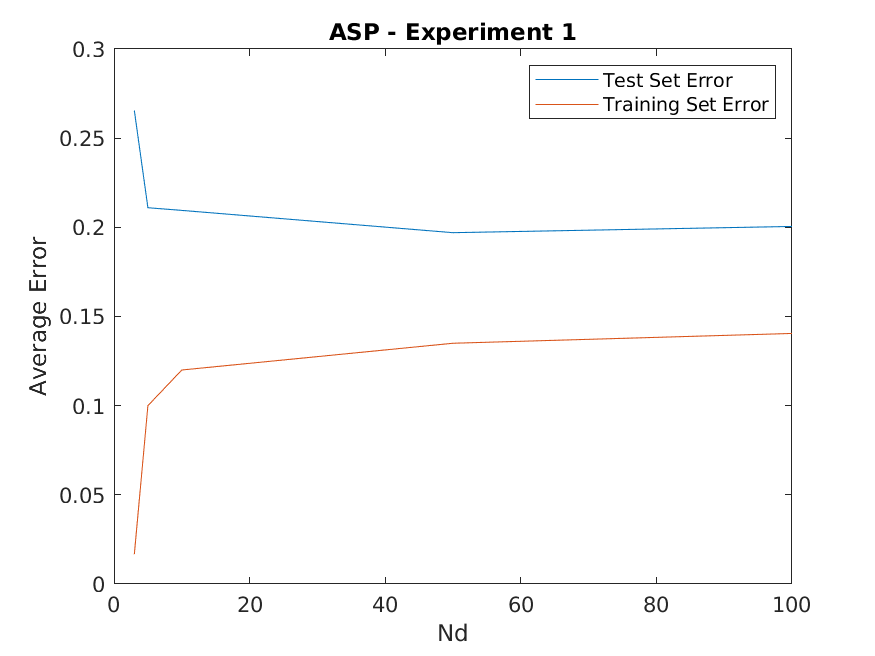
\includegraphics[width=.6\linewidth]{./code/Exp1-results/10iters/ErrorComparison.png}
	\caption{Experiment 1 Results}
	\label{fig:exp1}
\end{figure}


\subsection{Discussion}
